\documentclass[11pt,letterpaper]{article}

% include figures
\usepackage{graphicx}
% get nice colors
\usepackage{xcolor}

% change default font to Palatino (looks nicer!)
\usepackage[latin1]{inputenc}
\usepackage{mathpazo}
\usepackage[T1]{fontenc}
% load some useful math symbols/fonts
\usepackage{latexsym,amsfonts,amsmath,amssymb,wasysym}
% be able to insert code
\usepackage{listings}

% comfort package to easily set margins
\usepackage[top=1in, bottom=1in, left=1in, right=1in]{geometry}

% spacing after a paragraph
\setlength{\parskip}{.15cm}
% indentation at the top of a new paragraph
\setlength{\parindent}{0.0cm}
% make units not slanted in math mode
\newcommand{\unit}[1]{\ensuremath{\, \mathrm{#1}}}

\begin{document}

\begin{center}
\Large
Ay190 -- Worksheet 8\\
Daniel DeFelippis\\
Date: \today
\end{center}

%%
%%
%% I worked with Scott Barenfeld
%%
%% All python code can be found in the ws8 directory in my repository
%%
%%

\section*{ODE Integration: Simplified Stellar Structure}

We are solving two equations here:
\begin{align*}
\frac{dP}{dr} &= -\frac{GM(r)}{r^2}\rho(r) \\
\frac{dM}{dr} &= 4\pi \rho(r) r^2
\end{align*}
which are the equations of Hydrostatic Equilibrium and Mass
Conservation respectively. We also have the polytropic equation of state (EOS):
$$ P = K\rho^{\Gamma} $$
where 
\begin{align*}
K &= 1.224 \times 10^{15}(0.5)^{\Gamma} \unit{dyne \hspace{2pt} cm^{-2} (g^{-1}cm^{3})}^{\Gamma} \\
\Gamma &= 4/3
\end{align*}


\section{}

First, I'll describe the structure of the provided code. It begins be defining some 
constants, and then by defining two functions. The first function simply calculates
the right hand sides (RHS) of the two equations above for P and M, with the pressure
equation being the first in the tuple, and the equation for mass the second. The second 
function calculates the next step in forward Euler Integration by simply adding 
the RHS at step $n$ times the step size (in the code called $dr$) to the values of
pressure $P$ and mass $M$ at step $n$ to get the values of $P$ and $M$ at step $n+1$. 
After defining the step size and max radius, setting up the arrays for 
all of the variables, choosing initial values for the variables, and picking a 
minimum pressure to define the surface of the star, the program applies the 
Euler Integration function "npoints-1" number of times. Each time, it checks to make
sure that the pressure hasn't gotten below the surface value, and when it has, 
it sets all subsequent values of all of the variables to their surface values. It also
must update the density at each step, since that is not directly changed by the 
Euler Integration function. Finally, it prints out the surface radius and total mass.


\section{}

I filled in the code in the appropriate places with the lines shown below:
\lstinputlisting[language=Python, firstline=25, lastline=26]{ws8.py}
\lstinputlisting[language=Python, firstline=43, lastline=43]{ws8.py}
\lstinputlisting[language=Python, firstline=69, lastline=69]{ws8.py}
\lstinputlisting[language=Python, firstline=106, lastline=106]{ws8.py}
The "[i]" on "npoints" in the fourth line above is there because I run the 
code on multiple values of "npoints", so "npoints" is now an iterable array 
instead of a constant. Trying npoints=1000 does indeed give me the values I expect:
\begin{align*}
R &= 1501.5015015 \unit{km} \\
M &= 1.45069352 \unit{M_{\astrosun}}.
\end{align*}


\section{}

Next, I add an RK2 (and RK3 and RK4) integrator. The main thing I have to be careful 
about here is that when I use the "tov\_RHS()" function, I plug in the appropriate
value for the density, which is dependent on the pressure and therefore is also 
altered by the $k_i$'s. I also need to make sure I update the density at each step as
in the Euler method, since the algorithm itself doesn't do that.

Implementing the three RK integrators, and comparing with the Euler method, we see
that they all do converge to a value of mass and radius with a small step size.

Mass ($\unit{M\astrosun}$):
\begin{center}
    \begin{tabular}{| l | l | l | l | l |}
    \hline
    npoints & Euler & RK2 & RK3 & RK4 \\ \hline
    1000 & 1.45069352 & 1.45749017 & 1.45742325 & 1.4574234 \\ \hline
    10000 & 1.45674507 & 1.45742406 & 1.4574234 & 1.4574234 \\ \hline
    100000 & 1.45735552 & 1.45742341 & 1.4574234 & 1.4574234  \\
    \hline
    \end{tabular}
\end{center} 

Radius (km):
\begin{center}
    \begin{tabular}{| l | l | l | l | l |}
    \hline
    npoints & Euler & RK2 & RK3 & RK4 \\ \hline
    1000 & 1501.5015015 & 1537.53753754 & 1535.53553554 & 1535.53553554  \\ \hline
    10000 & 1533.55335534 & 1537.15371537 & 1537.15371537 & 1537.15371537  \\ \hline
    100000 & 1536.85536855 & 1537.21537215 &  1537.21537215 & 1537.21537215  \\
    \hline
    \end{tabular}
\end{center} 

To check the convergence of these methods, we look at 
$$ Q = \frac{|M(h_3) - M(h_2)|}{|M(h_2) - M(h_1)|} $$
for each method, where M is the mass, and $h_1$, $h_2$, and $h_3$ are the step 
sizes $\frac{1}{1000 - 1}$, $\frac{1}{10000 - 1}$, and $\frac{1}{100000 - 1}$ 
respectively.

For an order 1, 2, 3, or 4, process, we know that for these three step sizes, 
$Q \approx 0.1$, $0.01$, $0.001$, and $0.0001$ respectively. So, comparing 
the values using the masses to these will tell us the order of the 
convergence rate. The results are in the table below.

\begin{center}
    \begin{tabular}{| l | l | l | l | l |}
    \hline
    & Euler & RK2 & RK3 & RK4 \\ \hline
    $Q_{Mass}$ & 0.100873993813 & 0.00989946532494 & 0.00287248840483 & 0.0422107139183 \\ \hline
    $Q_{Radius}$ & 0.103020974551 & 0.160638930334 & 0.0381025525179 & 0.0381025525179 \\ \hline
    Order (M, R) & (1st, 1st) & (2nd, 1st) &  (3rd, 2nd) & (2nd, 2nd) \\
    \hline
    \end{tabular}
\end{center} 

As expected, the mass convergence of the Euler method has a rate of 1, and that of the 
RK2 method has a rate of 2. Additionally, the RK3 method has a mass convergence rate
of 3. Here, things get weird. RK4 should have a mass convergence rate of 4, but 
doesn't here probably because of rounding errors of the small differences between
the masses (dividing by a small number). Also, the radius convergence rates 
look "incorrect" probably because the radius is the independent variable in 
this situation, so it converges differently than the mass or pressure would. 

\section{}

A plot of Mass, Density, and Pressure vs Radius is shown below. The Density and 
Pressure lines are shown on a log scale. The left y-axis, in units of density, can
be transformed to the units of pressure by using the EOS. 

\begin{figure}[bth]
\centering
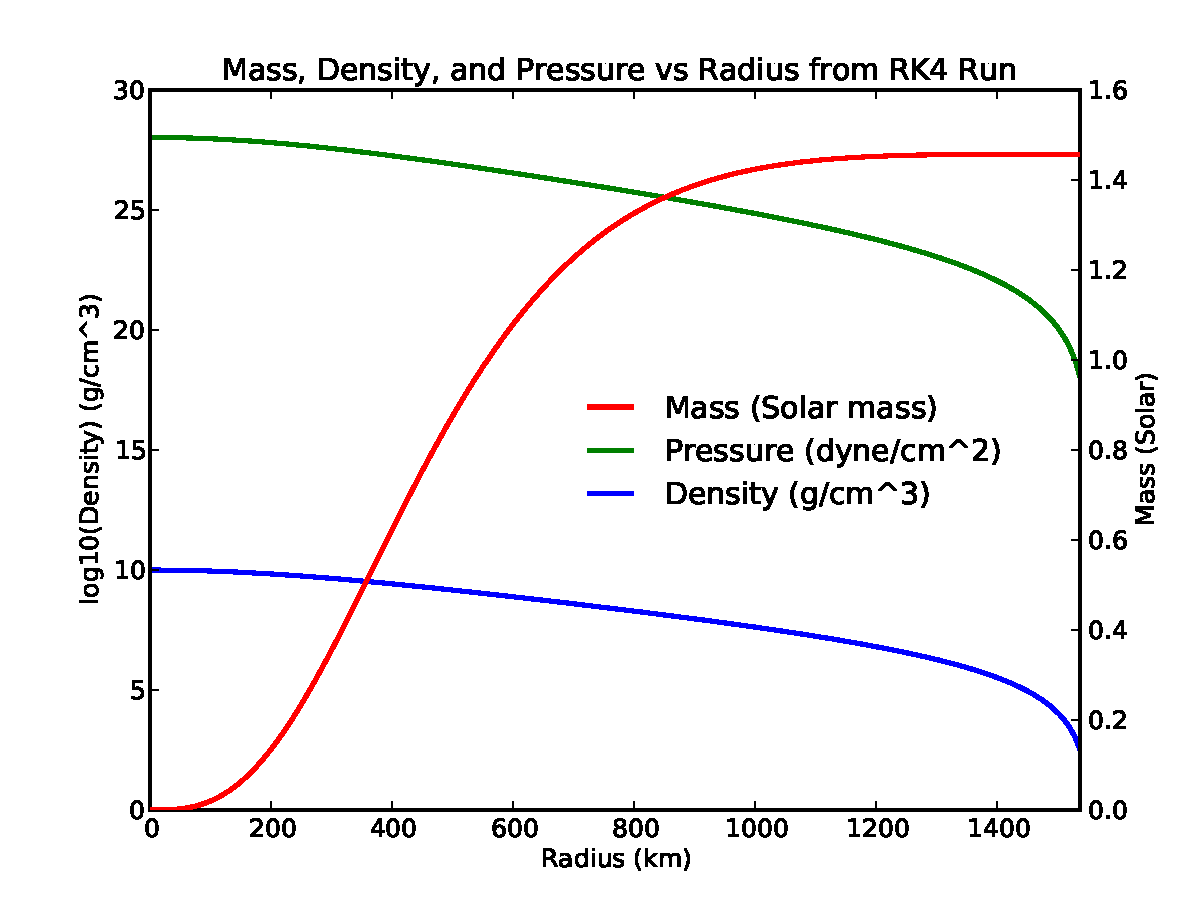
\includegraphics[width=0.95\textwidth]{MPrho.pdf}
\caption{Plot of $M$, $\log_{10}P$, and $\log_{10}\rho$ vs $R$ for the star}
\label{fig:MPrho}
\end{figure}

\end{document}
